%%%%%%%%%%%%%%%%%%%%%%%%%%%%%%%%%%%%%%%%%%%%%%%%%%%%%%%%%%%%%%%%%%%%%%%%
\cleardoubleevenemptypage
\chapter{The first scientific chapter}
\label{ch:pfff}
%%%%%%%%%%%%%%%%%%%%%%%%%%%%%%%%%%%%%%%%%%%%%%%%%%%%%%%%%%%%%%%%%%%%%%%%
\pgfmathsetmacro\chapclr{\colourarray[3]}
\hypersetup{
citecolor  = \chapclr,
linkcolor  = \chapclr,
urlcolor   = \chapclr,
}

\epigraph{
  A quasi-deep quote, with minimal relevance to the chapter.
  }{
    \textit{Piet J.M. Swinkels}
}

\begin{center}
    \begin{minipage}{\abstractwidth\textwidth}
      \begin{small}
        \blindtext[1]
      \end{small}
    \end{minipage}
    \vspace{0.5cm}
\end{center}

\clearpage
%%%%%%%%%%%%%%%%%%%%%%%%%%%%%%%%%%%%%%%%%%%%%%%%%%%%%%%%%%%%%

\section{Introduction}
\blindtext[2]
\section{Results}
\blindtext[1]
\blindmathpaper
\begin{figure}
  \centering
  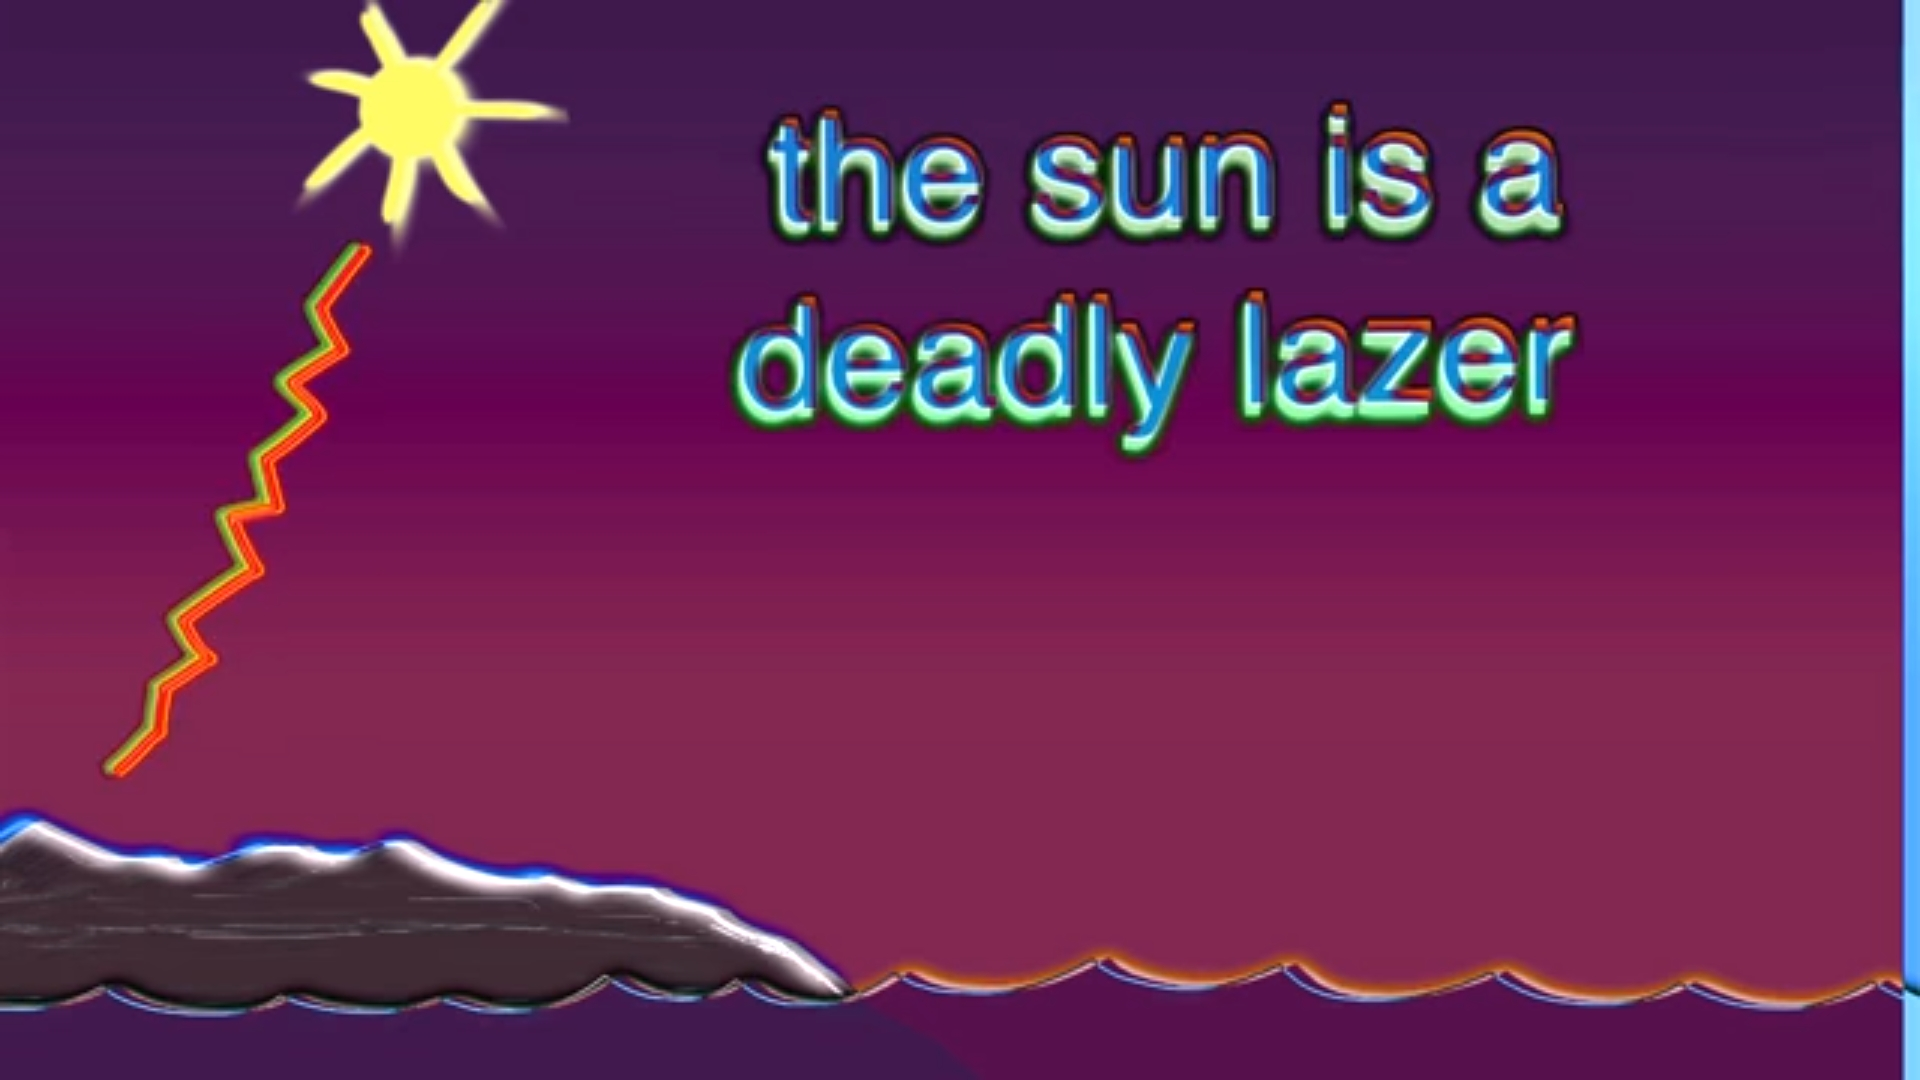
\includegraphics[width=1.0\linewidth]{Sections/Chapter3/Figures/laser.jpg}
  \caption{
    \textcolor{\chapclr}{Pewpewpew.}
    Cool stuff.
    }
  \label{fig:ch3-laser}
\end{figure}
\blindtext[1]
\section{Discussion}
\blindtext[2]

\clearpage

\section{Appendix}

\subsection{Sample preparation and history}

\blindtext[2]

\subsubsection{Math time!}

\blindtext[2]

The angular dependence of the interaction strength is captured by the switching function S which is a smoothly decaying function from 1 to 0 as shown in Figures \ref{fig:ch1-dog}\&\ref{fig:ch3-laser} on the right. We use the switching function

\begin{align}
  &S'(\Theta_i)=
  \begin{cases}
    \frac{1}{2} \left[ 1-\cos \left( \frac{\pi(\cos\Theta_i -\cos\Theta_\mathrm{p})}{1-\cos\Theta_\mathrm{p}} \right) \right]  &  \cos\Theta_i\geq \cos\Theta_\mathrm{p} \\
    0& \cos\Theta_i<\cos\Theta_\mathrm{p}
  \end{cases} \label{eq:ch3-switchfunction}
\end{align}
where $\Theta_\mathrm{p}$ is the patch arc-angle and $\cos\Theta_i=\vec{r_{ij}}\cdot\vec{p}_i/ |\vec{r}_{ij}\cdot\vec{p}_i|$ is the angle between the patch vector $\vec{p}_i$ and the interparticle vector $\vec{r}_{ij}$.